\section{Deferrable Work}

\subsection{Ausgangslage}

Ein System hat übermässig viele Anfragen. Um den korrekten Betrieb sicher zu stellen werden Routine Audits (24) und Routine Maintenance (22) angewandt. Durch die höhere Belastung des Systems treten aber keine Fehler auf, die behandelt werden müssen, lediglich die Ressourcen werden knapper.

\subsection{Lösungsansatz}

Ist ein System stabil und steht es vor einer Überlastung, kann es Sinn machen, die Prüfungen, welche Fehler verhindern sollen, später als geplant durchzuführen. Denn diese Routine-Checks sind nicht wichtig für das Abarbeiten der Anfragen. Das System soll sich bei einer Überlastung auf seine primäre Funktionalität konzentrieren.

\subsection{Schlussfolgerung}

Routinearbeit kann aufgeschoben (deferred) werden. Bei einem System, welches vor einer Überlastung steht, ist die Wahrscheinlichkeit gross, dass alle Komponenten richtig funktionieren. Die Routinearbeit soll dann wieder einsetzten, wenn die Ressourcen wieder vorhanden sind.

\begin{figure}[H]
	\centering
	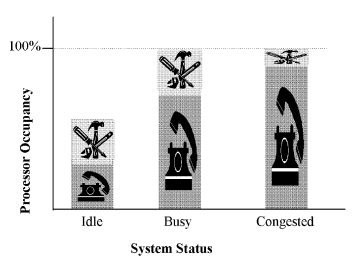
\includegraphics[width=\textwidth]{content/faulttolerance/images/DeferrableWork.JPG}
	\caption{DeferrableWork}
\end{figure}


\subsection{Verwandte Patterns}

Falls ein Fehler Überlastung verursacht:
\begin{itemize}
	\item Reasses Overload Decision (44)
\end{itemize}



